Almost every robot will rely on multiple sensors (including multiple \textit{types} of sensors) for perception and localization tasks. This allows the robot to take advantage of the different strengths of each sensor for a more well-rounded sensing capability. For example a self-driving car may use both laser rangefinders and radar for measuring distances, since in some cases one sensor may work better than the other. As another example, a wheeled robot may use GNSS sensors as well as wheel encoders to estimate position.
However, while each sensor may provide data toward a similar goal (e.g. estimating position or orientation) their sensing modalities may be drastically different. This chapter covers the topic of \textit{sensor fusion}\cite{Gustafsson2010}\cite{Simon2006}, and provides a discussion on algorithms for effectively leveraging multiple sensing modalities toward a common objective.

\notessection{Sensor Fusion}
Using measurements from multiple sensors (potentially different types of sensors) is an effective technique for reducing the uncertainty in downstream perception and estimation tasks (see Figure \ref{fig:reduceuncertainty}).
\begin{figure}[ht]
    \centering
    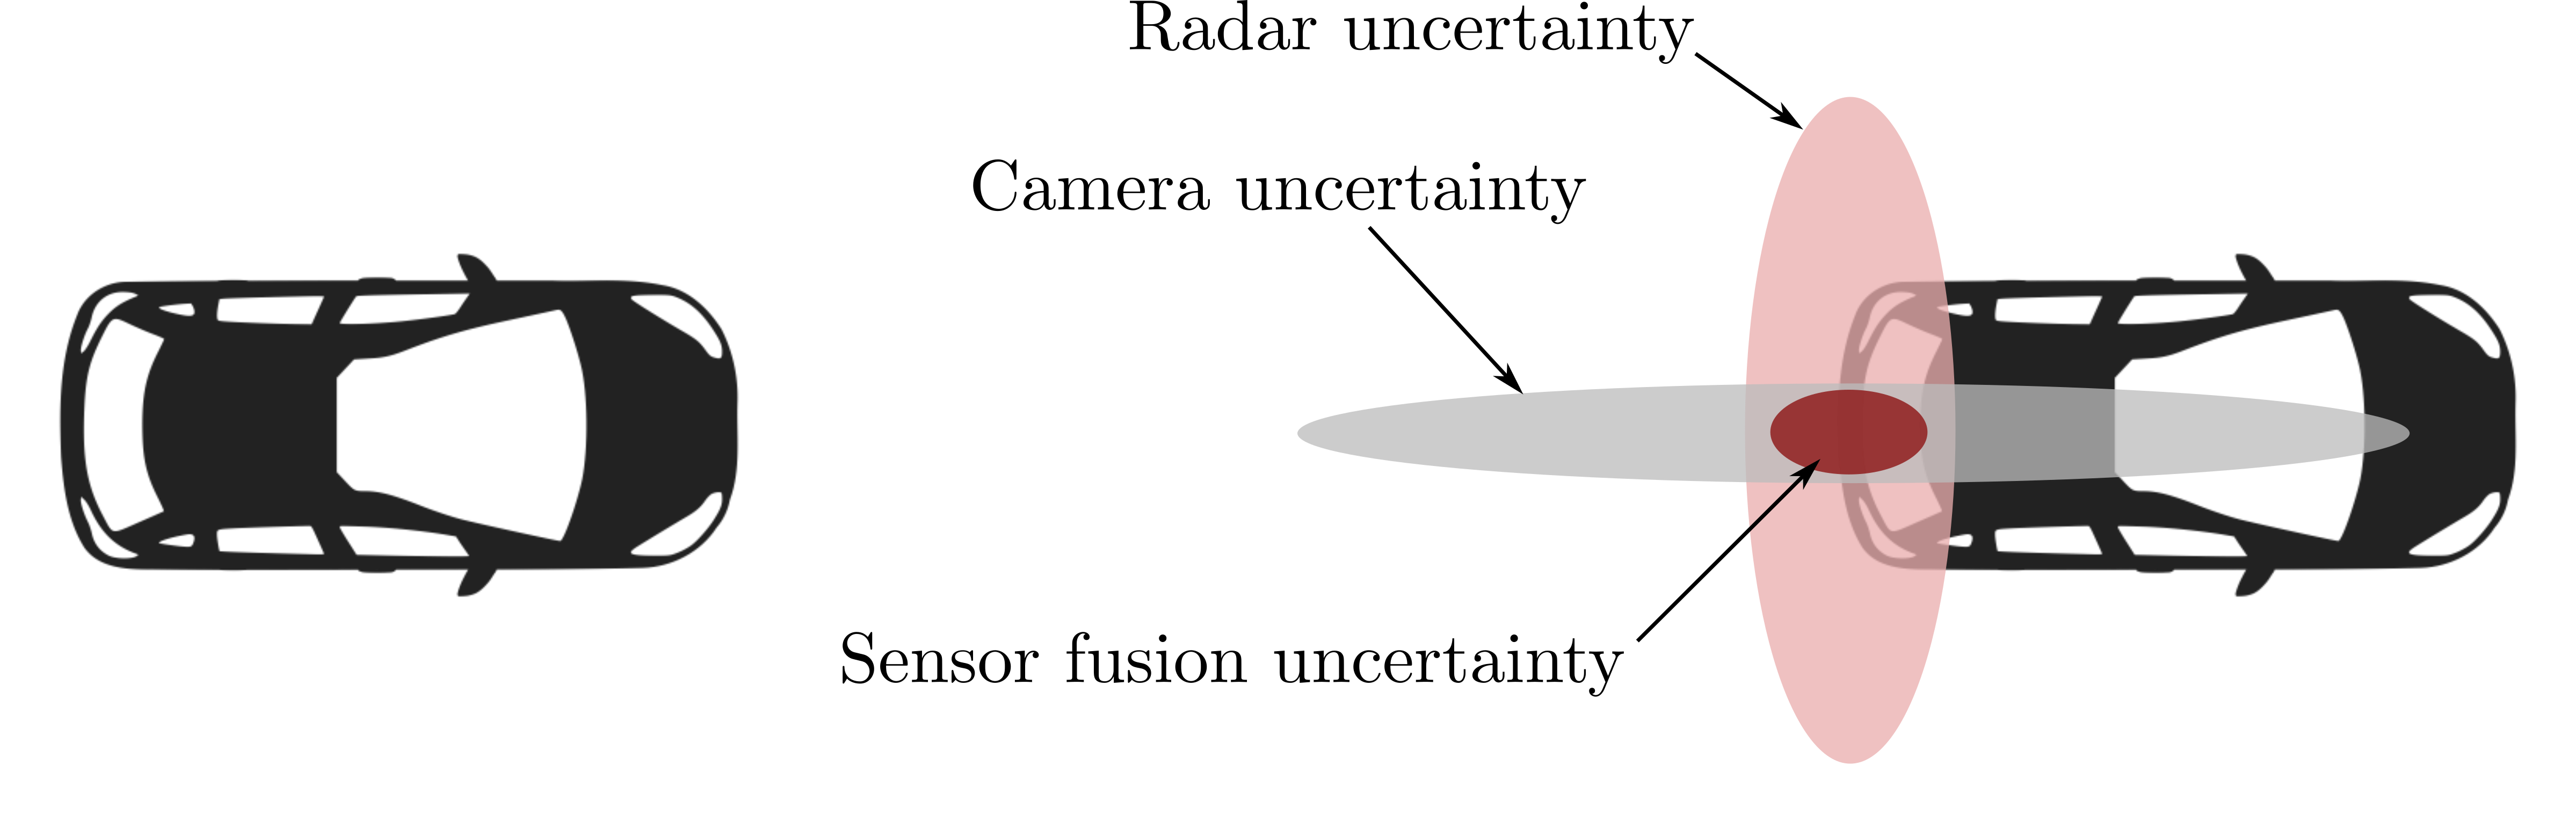
\includegraphics[width=0.85\textwidth]{tex/figs/ch19_figs/carsensors.png}
    \caption{Sensor fusion can reduce uncertainty by providing more well-rounded data. For example in this scenario the radar sensor may have good accuracy longitudinally but less accuracy laterally. Contrarily, a camera may provide poor range estimation but good lateral position estimation. By fusing these two sensor measurements the resulting estimate can be accurate both longitudinally and laterally.}
    \label{fig:reduceuncertainty}
\end{figure}
This is generally the case because individual sensors typically suffer from limited range, limited field of view, or performance degradation under certain environmental conditions. Additionally, in single-sensor systems measurement accuracy degradation and sensor failure can be catastrophic. Alternatively, multi-sensor systems can address these challenges through redundancy of individual sensors (e.g. to provide full field of view measurements or multiple measurements of the same quantity) or through sensor diversity (e.g. using sensors with different characteristics to offset limitations of others).


\subsection{A Taxonomy of Sensor Fusion}
To put the sensor fusion problem into a broader perspective, a taxonomy of sensor fusion related challenges will now be presented. This includes challenges associated with both fusion algorithms as well as the measurement data.

\subsubsection{Data-related Taxonomy}
One of the primary challenges with data fusion is the inherent imperfection in the measurement data, including uncertainty (i.e. resulting from sensor noise), imprecision (i.e. resulting from sensor bias), and granularity (i.e. resulting from sensor resolution). Other important data-related aspects to sensor fusion include data correlation, disparity, and inconsistency (e.g. data conflicts, outliers, disorder). Broadly speaking sensor data can experience multiple types of imperfection at the same time, and so data fusion algorithms should be developed with robustness in mind.

\subsubsection{Fusion-related Taxonomy}
At the data-fusion level, it is useful to classify the problem based on the type of data that is being fused. Low-level fusion problems typically fuse low-level signal data (i.e. time-series data), intermediate-level problems fuse features and characteristics, and high-level fusion problems consider decisions. Fusion problems can also be categorized based on the relationship among different sensors used in the fusion process. Competitive fusion problems consider redundant sensors that directly measure the same quantity. Complementary fusion is used when different sensors provide complementary information about the environment (e.g. lidar for short distance ranging and radar for long distance ranging). Finally, cooperative fusion considers problems where the required information cannot be inferred from a single sensor (e.g. GNSS localization and stereo vision can be cooperatively used because they measure fundamentally different environmental quantities). Generally speaking competitive fusion increases reliability and accuracy of fused information, complementary fusion increases the completeness of information, and cooperative fusion broadens the types of information that can be gathered.

\subsubsection{Architectural Taxonomy}
Fusion algorithms can also be classified based on their type of architecture, namely whether they are centralized, decentralized, or distributed. Centralized architectures collect \textit{all} sensor data first, and then perform computations on the entire set of data. This approach is theoretically optimal since all information is gathered and operated on at once, but the need for high levels of communication and processing can be challenging in practice. Decentralized architectures are essentially collections of centralized systems, and generally still suffer from the same high demands for communication and processing. On the other hand, distributed architectures do not collect all sensor information ahead of time but rather perform computations on local sensor data first, before potentially passing information on for further fusion tasks. These architectures scale better, but can lead to suboptimal performance because each sensor is performing local processing (i.e. without having all information).

\subsection{Bayesian Approach to Sensor Fusion}
Previous chapters presented several algorithms for robot state estimation and localization based on Bayes' filter. In fact, these algorithms can be viewed as approaches to solve the sensor fusion problem. This section explores the Bayesian approach to sensor fusion in more detail to show exactly how these approaches can blend measurement data to reduce uncertainty.

Recall that the Bayesian approach is a probabilistic approach that models unknowns as random variables and quantifies knowledge in the form of probability distributions over the unknowns. This principled approach is useful for sensors fusion for several reasons. First, it provides a unified framework for representing knowledge that is compatible with any quantity and type of sensors and is interpretable. Second, probability distributions implicitly provide information about uncertainty (e.g. the variance of a Gaussian). Third, Bayes' rule provides a principled approach for updating distributions. Finally, they can be used to deal with missing information and classification of new observations.

\begin{example}[Competitive Fusion Example] \label{ex:competitive}
\theoremstyle{definition}
As an example to show how a probabilistic approach can be used to reduce uncertainty through sensor fusion, consider a case where two sensors are fused to estimate a single quantity $x\in \R$. Specifically, suppose the two measurements $y_1$ and $y_2$ are normally distributed random variables:
\begin{equation*}
\begin{split}
p(y_1 \mid x) &= \frac{1}{\sqrt{2\pi \sigma_1^2}} e^{-\frac{1}{2}\frac{(x-y_1)^2}{\sigma_1^2}}, \\ 
p(y_2 \mid x) &= \frac{1}{\sqrt{2\pi \sigma_2^2}} e^{-\frac{1}{2}\frac{(x-y_2)^2}{\sigma_2^2}}, \\ 
\end{split}
\end{equation*}
where the first sensor has a higher precision than the second sensor such that $\sigma_1^2 < \sigma_2^2$. Then the \textit{combined} measurement probability is given by:
\begin{equation*}
p(y_1, y_2 \mid x) = p(y_1 \mid x)p(y_2 \mid x),
\end{equation*}
by assuming conditional independence. By exploiting the product of two Gaussian property this joint probability distribution is:
\begin{equation*}
p(y_1, y_2 \mid x) = \frac{1}{\sqrt{2\pi \sigma^2}} e^{-\frac{1}{2}\frac{(x-\mu)^2}{\sigma^2}},
\end{equation*}
where:
\begin{equation*}
\mu = \frac{y_1\sigma_2^2 + y_2\sigma_1^2}{\sigma_1^2 + \sigma_2^2}, \quad \sigma = \frac{\sigma_1^2 \sigma_2^2}{\sigma_1^2 + \sigma_2^2}.
\end{equation*}
Therefore, given two measurements $y_1$ and $y_2$ the best estimate of the quantity $x$ is given by $\mu$, which is a \textit{weighted} average of the two measurements. In particular, more weight is given to the measurement with higher precision (i.e. higher variance $\sigma_i^2$) and the overall uncertainty will decrease!
\end{example}


\subsubsection{Kalman Filter Sensor Fusion}
The Kalman filter from the previous chapter on parametric state estimation techniques is a common tool for sensor fusion problems. Recall that the Kalman filter assumes a linear state transition (dynamics) model:
\begin{equation} \label{eq:KFSFdynamics}
    \x_t = A_t \x_{t-1} + B_t \bu_t + \bm{\epsilon}_t,
\end{equation}
and a linear measurement model:
\begin{equation} \label{eq:KFSFmeasure}
\z_t = C_t \x_t + \bm{\delta}_t,
\end{equation}
where $\x$ is the state of the system and $\z$ are the measurements. Additionally, the Kalman filter assumes the belief distribution of $\x$ and the noise terms $\bm{\epsilon}$, $\bm{\delta}$ are all Gaussian:
\begin{equation*}
bel(\x_t) \sim \mathcal{N}(\bmu_t, \bSigma_t), \quad \bm{\epsilon}_t \sim \mathcal{N}(\bm{0}, \bm{R}_t), \quad \bm{\delta}_t \sim \mathcal{N}(\bm{0}, \bm{Q}_t),
\end{equation*}
where $\bm{R}_t$ and $\bm{Q}_t$ are the covariances of the state transition and measurement noise models, respectively.
With these assumptions the Kalman filter algorithm uses a recursive ``predict then correct'' approach and the belief will always remain normally distributed.

This algorithm can be used for sensor fusion since the measurement vector $\z$ can include measurements from any type of sensor, as long as a linear relationship exists between the measurement and the underlying state $\x$ that is to be estimated. At each step of the Kalman filter algorithm, \textit{every} measurement at time $t$ is simultaneously used to update or ``correct'' the state predicted from the state transition model. Additionally, the Kalman filter takes into account the covariance $\bm{R}_t$, which includes the covariance of each individual sensor. In fact, the Kalman filter will implicitly favor measurements with lower covariance when performing the correction step\footnote{Specifically, this occurs during the computation of the Kalman gain.}.

A useful trick for applying the Kalman filter to sensor fusion problems is to also note that the state $\x$ can contain any type of information, it is not strictly limited to the state usually associated with the robot's dynamics or kinematics. For example, the state could be augmented with auxiliary states such as sensor bias or offsets, or variables to define sensor and actuator health.


\begin{example}[Kalman Filter Multi-Sensor Fusion Example] \label{ex:car}
\theoremstyle{definition}
Consider a self-driving car that has an inertial measurement unit (IMU), a GNSS receiver, and a Lidar unit and where the goal is to leverage all of these sensors to estimate the position, velocity, and acceleration of the vehicle. This suite of sensors can provide noisy position estimates (Lidar and GNSS) as well as noisy acceleration measurements (IMU).
For this application, sensor fusion can be accomplished through a Kalman filter.

First, consider a very simple kinematics model that only models longitudinal motion:
\begin{equation*}
\dot{p} = v, \quad \dot{v} = a,
\end{equation*}
where $p$ is the longitudinal position, $v$ is the longitudinal velocity, and $a$ is the longitudinal acceleration. This model is then discretized in time by choosing a sampling time $T_s$, yielding the linear difference equation:
\begin{equation*}
\begin{bmatrix}
p_{t+1} \\ v_{t+1} \\ a_{t+1}
\end{bmatrix} = \begin{bmatrix}
1 & T_s & \frac{T_s^2}{2} \\
0 & 1 & T_s \\
0 & 0 & 1
\end{bmatrix}\begin{bmatrix}
p_{t} \\ v_{t} \\ a_{t}
\end{bmatrix} + \bm{\epsilon}_t,
\end{equation*}
where the state is defined as $\x = [p, v, a]^T$, and $\bm{\epsilon}$ is Gaussian process noise.

It is assumed that the lidar and GNSS sensors directly measure the position $p$, and that the IMU directly measures the acceleration $a$, such that the measurement model is:
\begin{equation*}
\begin{bmatrix}
z_{\text{lidar},t} \\ z_{\text{gnss},t} \\ z_{\text{imu},t}
\end{bmatrix} = \begin{bmatrix}
1 & 0 & 0 \\
1 & 0 & 0 \\
0 & 0 & 1
\end{bmatrix}\begin{bmatrix}
p_{t} \\ v_{t} \\ a_{t}
\end{bmatrix} + \bm{\delta}_t,  
\end{equation*}
where $\bm{\delta}$ is Gaussian measurement noise with zero mean and covariance:
\begin{equation*}
\bm{Q}_t = \begin{bmatrix}
\sigma_{\text{lidar}}^2 & 0 & 0 \\
0 & \sigma_{\text{gnss}}^2 & 0 \\
0 & 0 & \sigma_{\text{imu}}^2
\end{bmatrix},
\end{equation*}
with $\sigma_{\text{lidar}} = 0.5$, $\sigma_{\text{gnss}} = 0.1$, and $\sigma_{\text{imu}} = 0.2$

Figure \ref{fig:fusionexample} shows results of the application of the Kalman filter algorithm for fusing these sensor measurements into position estimates. The top plot presents a case where the GNSS sensor is not used, and as can be seen the noisy high-variance lidar measurements result in a noisy estimate of the ground truth position of the car. However, with the addition of the lower-variance GNSS sensor in the bottom figure, the estimate of the position is much more accurate. Generally speaking the estimate would also be more accurate even with the addition of a sensor that was even more noisy than the lidar, but the impact would not be as significant.

\begin{figure}[ht!]
    \centering
    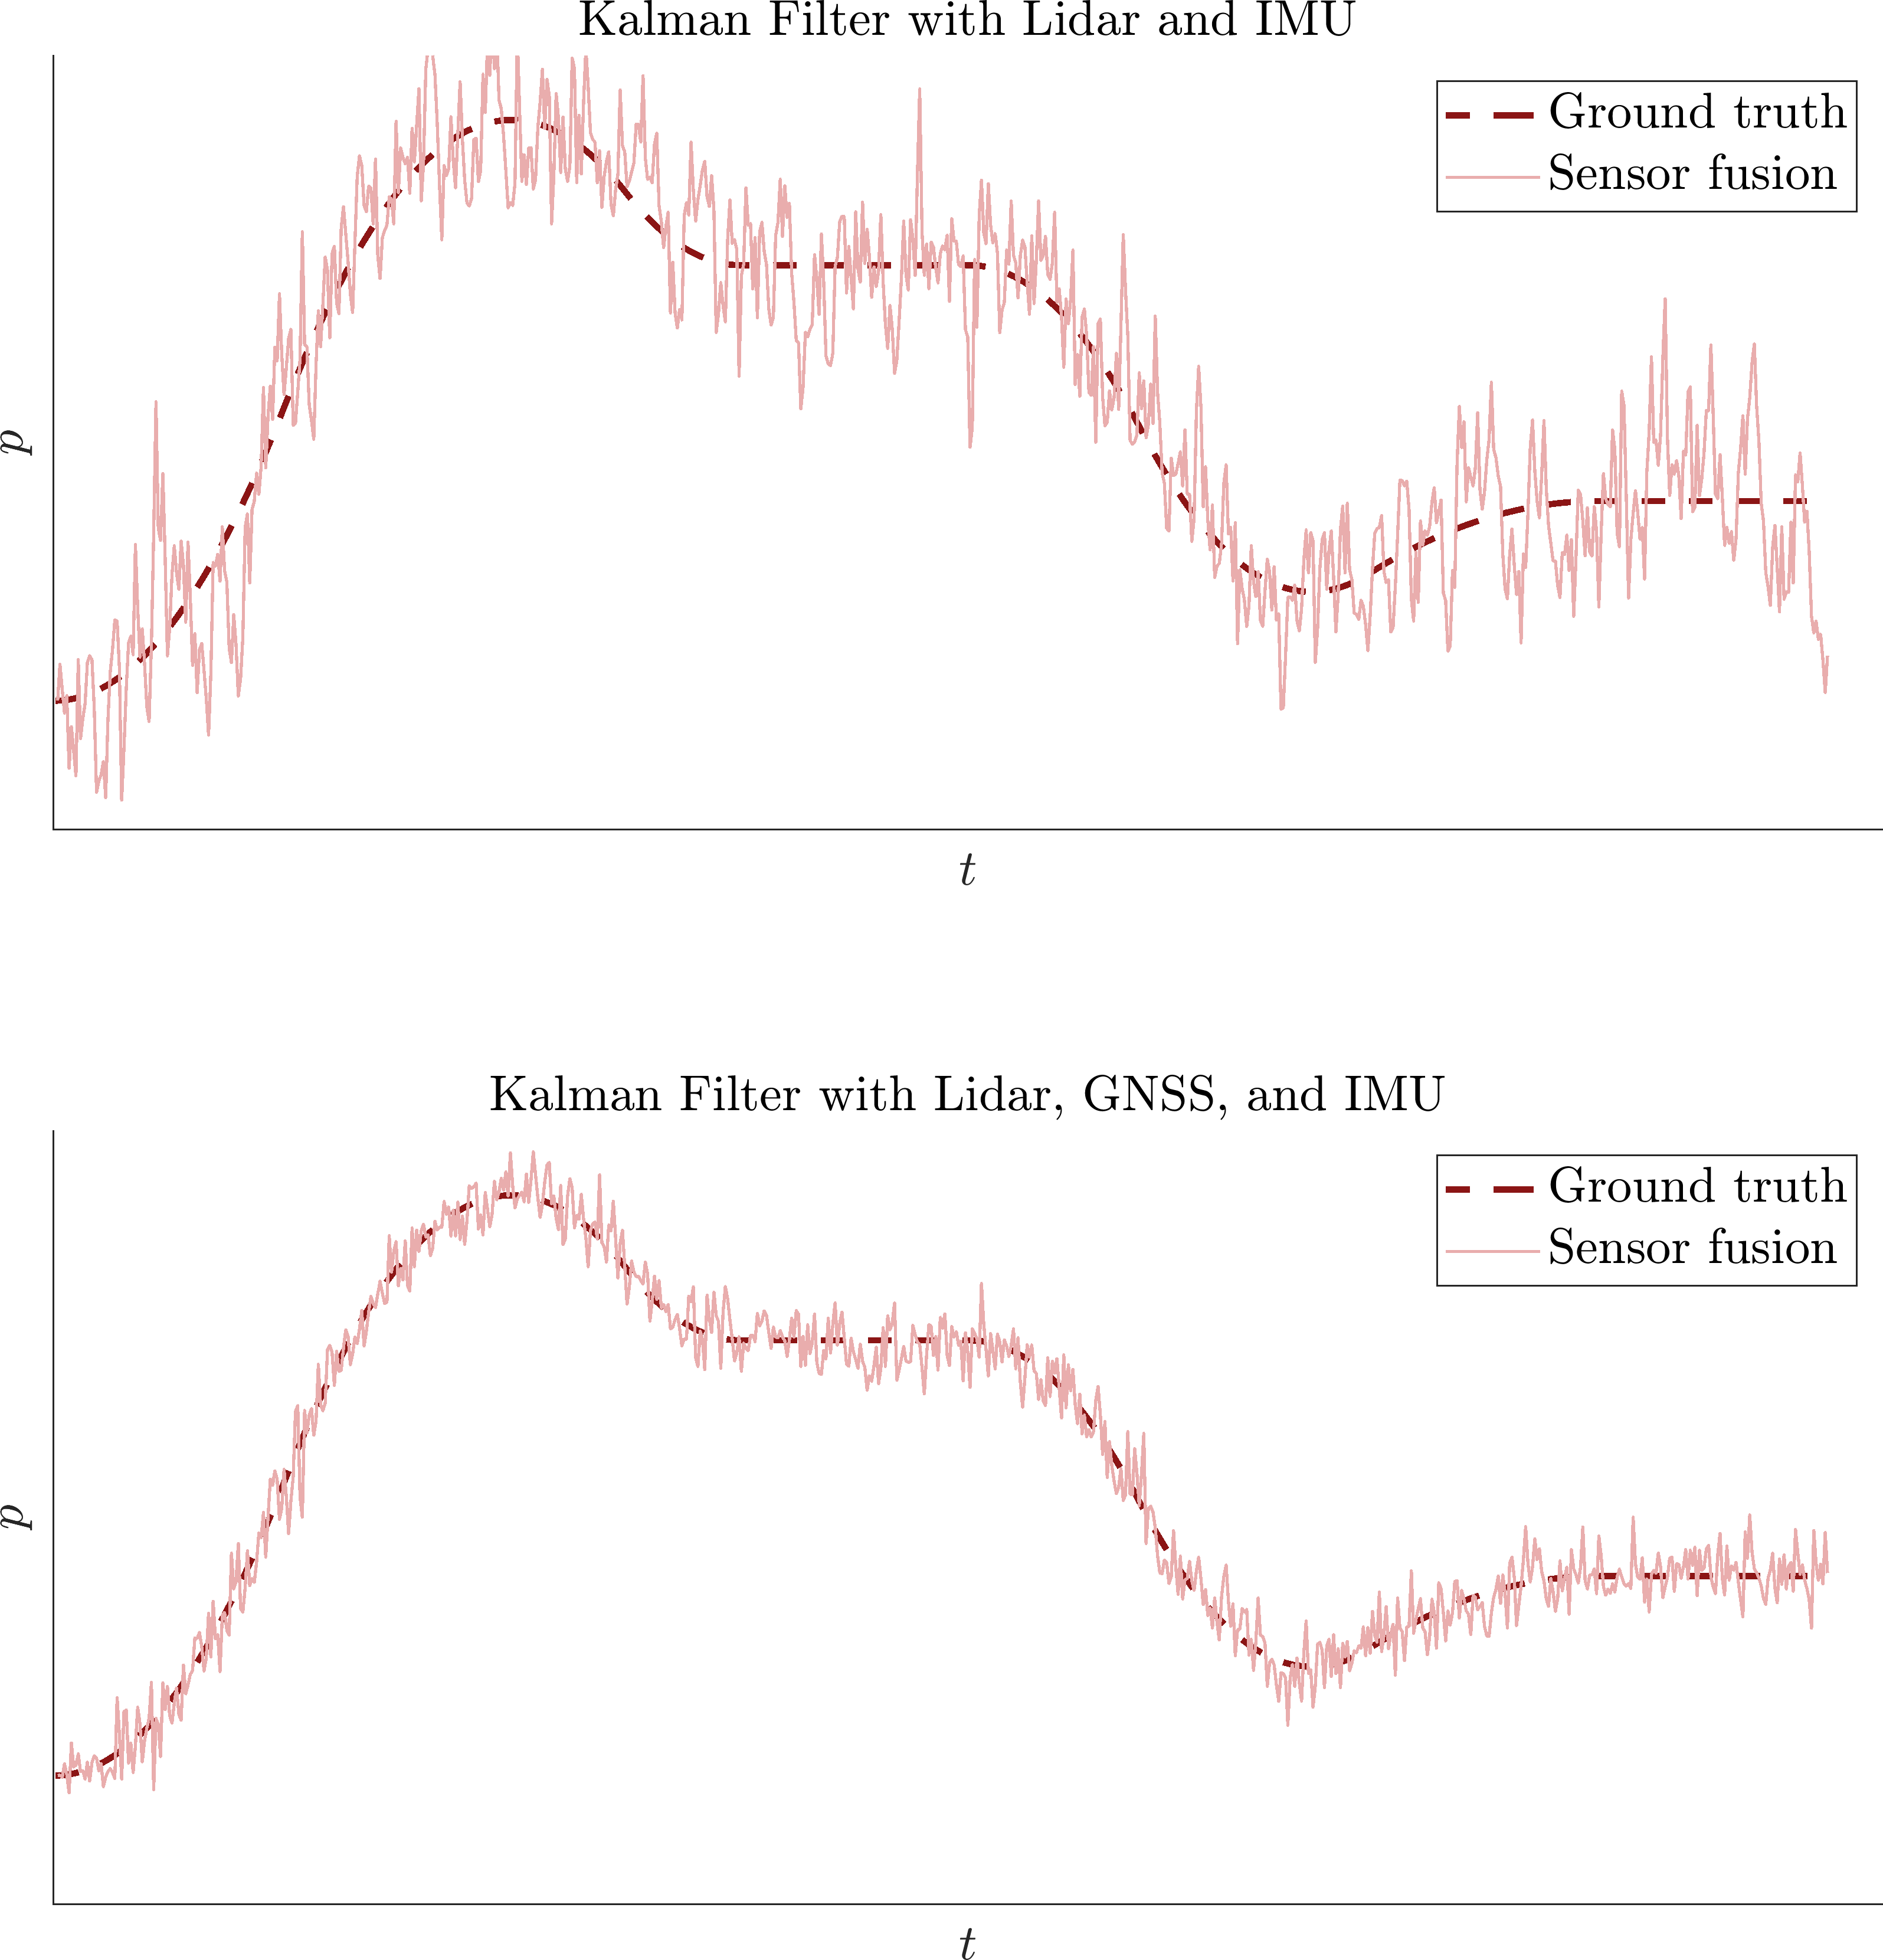
\includegraphics[width=0.85\textwidth]{tex/figs/ch19_figs/carKFfusion.png}
    \caption{Kalman filter sensor fusion for Example \ref{ex:car}. The position of a vehicle is estimated using noisy lidar, GNSS, and IMU data, and the resulting estimate tracks the ground truth. As can be seen, the addition of the lower-variance GNSS results in a better estimate through sensor fusion.}
    \label{fig:fusionexample}
\end{figure}
\end{example}


\subsection{Challenges in Sensor Fusion}
Sensor fusion problems can generally be quite challenging, and can vary significantly from application to application. Some of the more common problems in sensor fusion include registration, bias, correlation, data association, and out-of-sequence measurements.
The registration problem is that coordinates (both time and space) of different sensors may not always be aligned, which is necessary to ensure they can be appropriately combined. Biases can also arise due to transformations of the data into the unified set of coordinates. Correlation between sensors can also occur, even if they are independently collecting data, and the knowledge of correlation between sensors can have an impact on the best way to fuse the information. In some robotics applications, data association can also be a challenge. One simple example is in multi-target tracking problems, which is similar to the correspondence problem in SLAM problems. Finally, out-of-sequence measurements also pose a logistical challenge in practical sensor fusion applications. These issues often arise due to communication limitations among agents in multi-agent settings.